共享數據的併發(同時)訪問是一個性能殺手。因為為了避免數據競爭,在給定的時間內只有一個線程可以操作共享數據。可以使用互斥量來完成這個任務,如果有原子操作的話,可以使用原子操作。無論哪種方式,當一個線程遞增共享變量時,其他所有線程都必須等待。上一節的測試結果也證實了這一點。

然而,在根據觀察和測試採取任何行動前,要理解我們測試了什麼,以及可以確定地得出什麼結論。

多個線程同時遞增一個共享變量根本沒有擴展性,甚至比只使用一個線程還要慢,原子共享變量和互斥保護的非原子變量都是如此。這裡沒有嘗試測試對非原子變量的無保護訪問,因為這樣的操作會導致未定義行為和不正確的結果。對特定於線程(非共享)變量的無保護訪問,可以很好地隨著線程的數量而擴展,至少在飽和了內存帶寬前是這樣(這隻會發生在寫大量數據的時候;對於單個變量來說,這不是問題)。批判性地、不帶偏見地分析實驗結果是一項重要的技能,有保護的訪問共享數據很慢,而無保護的訪問非共享數據很快。如果由此得出共享數據會使程序變慢的結論,就需要做出一個假設:\textbf{共享數據}重要,而\textbf{訪問保護}不重要。這就引出了在進行性能測量時的另一個問題:比較程序的兩個版本時,一次只更改其中一個的內容,然後測試結果。

我們缺少對受保護數據的非共享訪問的衡量標準。當然,這裡不需要保護單線程的數據訪問,但我們試圖理解是什麼原因使共享數據的訪問有如此大開銷。是共享或是原子的原因(或由鎖保護)?為了確定這一點,需要一次做一個更改,所以保持原子訪問並刪除數據共享。第一種方法是創建一個原子變量的全局數組,並讓每個線程訪問自己的數組元素:

\hspace*{\fill} \\ %插入空行
\noindent
\textbf{04\_local\_incr.C}
\begin{lstlisting}[style=styleCXX]
std::atomic<unsigned long> a[1024];
void BM_false_shared(benchmark::State& state) {
	std::atomic<unsigned long>& x = a[state.thread_index];
	for (auto _ : state) {
		benchmark::DoNotOptimize(++x);
	}
}
\end{lstlisting}

谷歌基準測試中的線程索引對於每個線程都是唯一的,數字從0開始,並且是緊湊的(0,1,2…)。另一種簡單的方法是在基準函數中聲明變量,如下所示:

\hspace*{\fill} \\ %插入空行
\noindent
\textbf{04\_local\_incr.C}
\begin{lstlisting}[style=styleCXX]
void BM_not_shared(benchmark::State& state) {
	std::atomic<unsigned long> x;
	for (auto _ : state) {
		benchmark::DoNotOptimize(++x);
	}
}
\end{lstlisting}

現在,對同一個原子整數進行遞增,就像為圖5.4收集測試數據時所做的那樣,只是現在不再在線程之間共享。這將說明性能變差是共享的原因,還是原子變量的原因。以下是結果:

%\hspace*{\fill} \\ %插入空行
\begin{center}
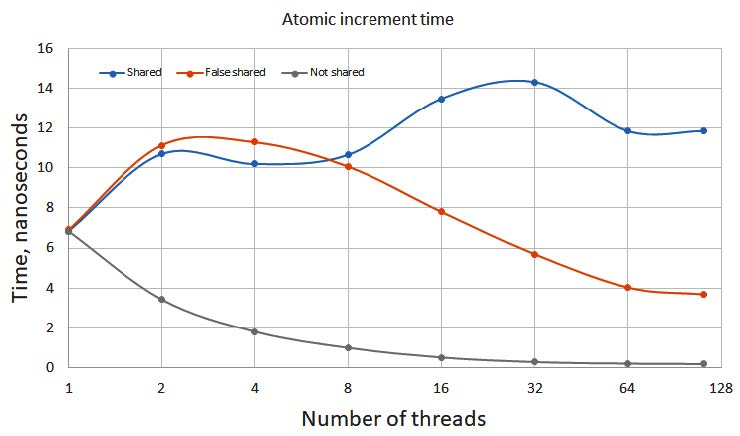
\includegraphics[width=0.9\textwidth]{content/1/chapter5/images/6.jpg}\\
圖5.6 - 共享和非共享變量的原子增量時間
\end{center}

圖5.4中的的\textbf{Shared}曲線為共享數據的曲線,另外兩條曲線為不共享數據的曲線。線程上都有一個局部變量的基準測試標記為\textbf{Not shared}。在兩個線程上的計算時間比在一個線程上的計算時間少一半,在四個線程上的計算時間又減少了一半,以此類推。請記住,這是一個增量操作的平均時間,總共做了100萬次增量計算,測試它所花費的總時間,然後除以100萬。由於遞增的變量不是在線程之間共享的,所以期望兩個線程的運行速度是一個線程的兩倍,所以\textbf{Not shared}的結果與期望相符。另一個基準測試中,使用原子變量數組,但每個線程使用自己的數組元素,也沒有共享數據。然而,其執行就像數據在線程之間共享一樣,至少對於少量的線程是這樣,所以稱它為\textbf{偽共享}:沒有什麼是真正共享的,但程序的行為就像是共享的一樣。

這個結果表明,數據共享成本高的原因比之前假設的要複雜。在偽共享的情況下,只有一個線程在操作每個數組元素,所以不需要等待任何其他線程完成其增量操作。然而,線程顯然在彼此等待。為了理解這種異常現象,必須對緩存的工作方式進行更多的瞭解。

在多核或多處理器系統中,數據在處理器和內存之間移動的方式如圖5.7所示。

%\hspace*{\fill} \\ %插入空行
\begin{center}
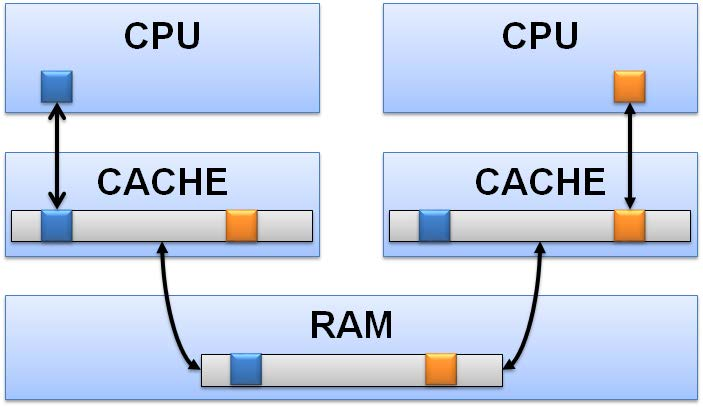
\includegraphics[width=0.6\textwidth]{content/1/chapter5/images/7.jpg}\\
圖5.7 - 多核系統中CPU和內存之間的數據傳輸
\end{center}

處理器以字節或整數的形式處理數據,這取決於變量的類型。在我們的例子中,一個\texttt{unsigned long}類型變量具有8字節。原子增量讀取指定地址處的單個字,對其加1,然後寫回。但是從哪裡讀呢?CPU只能直接訪問L1緩存,因此只能從那裡獲取數據。數據如何從主存儲器進入高速緩存?數據是通過內存總線複製的,而內存總線要寬得多。可以從內存複製到高速緩存並返回的最小數據量稱為\textbf{緩存行}。在所有x86 CPU上,一條緩存行的大小為64字節。當CPU需要為一個原子事務鎖定內存位置時,比如一個原子增量,CPU可能在寫一個數據,並鎖定整個緩存行:如果兩個CPU可以在同一時間將同一緩存行寫入內存,那麼其中一個必然會覆蓋另一個。注意,為了簡單起見,在圖5.7中只顯示了一個級別的緩存層次結構,但這沒有區別。數據會以緩存行長的形式經過所有級別的緩存。

現在可以解釋我們觀察到的偽共享。即使相鄰的數組元素在線程之間並沒有真正共享,但確實佔用了相同的緩存行。當CPU請求獨佔訪問一個數組元素時,會鎖定整個緩存行,阻止其他CPU訪問其中的任何數據。這也解釋了為什麼圖5.7中的偽共享在8個線程時看起來和真正的數據共享是一樣的,但是在更多的線程時變得更快:寫入的是8個字節的數據,所以它們中的8個可以放進同一個緩存行中。如果只有8個線程(或更少),那麼在任何給定的時間,只有一個線程可以增加它的值,這與真正的共享一樣。但是如果超過8個線程,數組至少佔用兩條緩存行,並且可以被兩個獨立的CPU鎖住。所以,若有16個線程,那麼就有兩個線程可以向前移動,數組的一半對應一個線程。

另一方面,真正的非共享基準測試在每個線程的堆棧上分配原子變量。是完全獨立的內存分配,由許多緩存行隔開。由於沒有內存交互,這些線程可以完全獨立地運行。

分析表明,訪問共享數據的高成本的真正原因是,必須維護對緩存行的獨佔訪問,並確保所有CPU的緩存中有一致的數據。當一個CPU獲得了獨佔訪問權,並且更新了緩存行上的1位後,所有其他CPU的緩存行副本就過期了。在其他CPU訪問同一緩存行的數據之前,必須從主存中獲取更新後的內容,這將花費較長的時間。

兩個線程是否訪問相同的內存位置並不重要,重要的是它們會競爭訪問相同的緩存行。獨佔的緩存行訪問是共享變量高成本的根源。

有人可能想知道,鎖昂貴的原因是否也存在於包含的共享數據中(所有鎖都必須具有一定數量的共享數據,這是一個線程可以讓另一個線程知道鎖佔用的唯一方法)。即使是在一個線程上,互斥鎖也比單個原子訪問要昂貴得多,如圖5.4和5.5中看到的那樣。鎖定互斥對象比僅僅修改一個原子變量需要更多的工作。但是,當有多個線程時,為什麼這項工作要花費更多的時間呢?是因為數據是共享的,需要獨佔的訪問緩存行嗎?我們把這個問題留給讀者作為一個練習,通過自己的方法確認是否真的是這樣。這個問題的關鍵是設置鎖的偽共享。一個鎖數組,每個線程操作自己的鎖,競爭相同的緩存行(當然,這種每個線程的鎖實際上並不能保護併發訪問,但我們想要的是鎖定和解鎖所花費的時間)。標準C++的互斥量\texttt{std::mutex}通常相當大,根據操作系統的不同,在40到80字節之間,可能不能在同一個緩存行中放入兩個互斥量。所以必須使用較小的鎖來進行這個實驗,例如:自旋鎖或futex(fast userspace mutex)。

現在明白了為什麼併發訪問共享數據的代價如此之高。這裡需要注意兩點:首先,創建非共享數據時,要避免錯誤的數據共享。無意間的錯誤共享會在程序出現嗎?這一章已經有了個簡單的例子:對多個數進行同時累加求和。我們的方法都非常慢(比單線程程序慢,或者和單線程性能相當),同時也清楚了訪問共享數據的開銷很高。那麼,有什麼方法能降低這個開銷呢?當然,不是訪問共享數據!至少是不經常訪問它。對於我們來說,不需要在想要進行累加時,就訪問共享內存。我們可以在本地、線程上進行累加,並在最後一次性將它們添加到共享的累加值中:

\hspace*{\fill} \\ %插入空行
\noindent
\textbf{04\_local\_incr.C}
\begin{lstlisting}[style=styleCXX]
// Global (shared) results
std::atomic<unsigned long> sum;
unsigned long local_sum[…];
// Per-thread work is done here
unsigned long& x = local_sum[thread_index];
for (size_t i = 0; i < N; ++i) ++x;
sum += x;
\end{lstlisting}

我們有一個全局結果\texttt{sum},它在所有線程之間共享,並且必須是原子的(或者由鎖保護)。但是在所有的工作完成後,每個線程只訪問這個變量一次。每個線程使用另一個變量來保存部分和,只保存在該線程上添加的值(在我們的簡單示例中,增量為1,但無論添加的值是什麼,性能都是相同的)。我們可以創建一個大數組來存儲每個線程的部分和,並給每個線程一個單獨的數組來對元素進行處理。在這個簡單的例子中,可以只使用一個局部變量,但是在實際的程序中,部分結果通常需要在工作線程完成之後保存,而這些結果的最終處理可能是通過其他線程完成的。為了模擬這種實現,我們使用每個線程的數組。注意,這些數組中只是普通的整數:不會併發訪問。在此過程中,我們落入了錯誤共享的陷阱:數組的相鄰元素(通常)位於同一高速緩存行上,因此不能併發訪問。這反映在程序的性能上:

%\hspace*{\fill} \\ %插入空行
\begin{center}
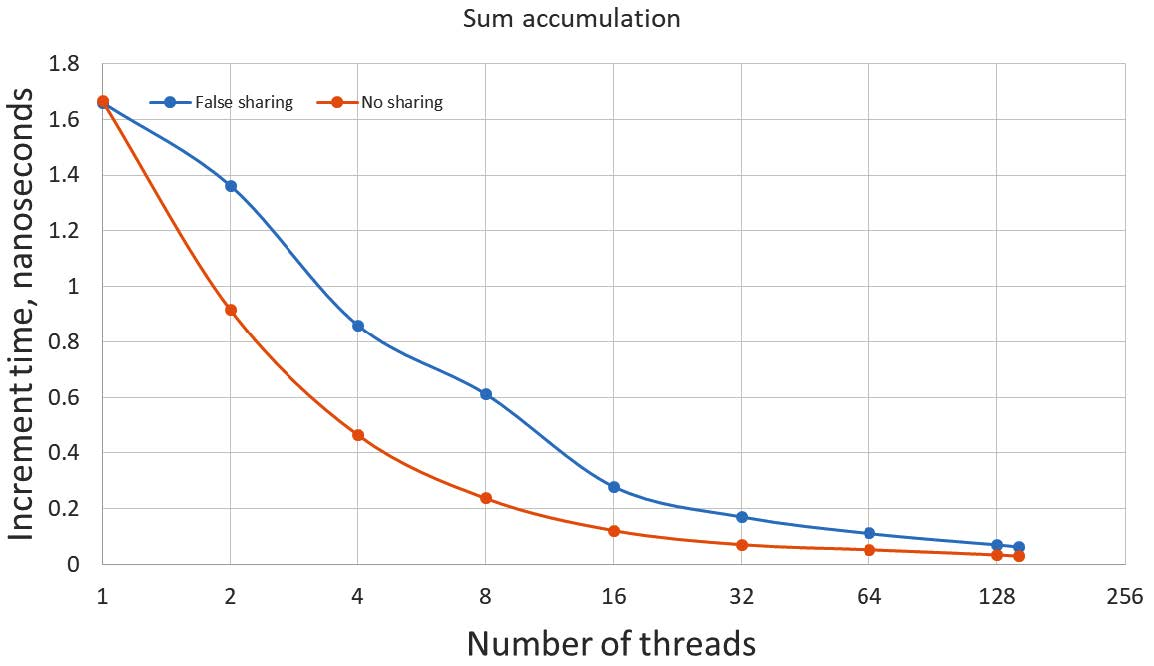
\includegraphics[width=0.9\textwidth]{content/1/chapter5/images/8.jpg}\\
圖5.8 - 有與沒有偽共享的累加計算
\end{center}

可以在圖5.8中看到,程序的擴展性非常差,需要開非常多的線程才會好。另一方面,如果通過確保每個線程的部分和之間,至少有64字節(或者在我們的例子中僅使用局部變量)來消除偽共享,那麼就可以完美地擴展。當使用更多的線程時,兩個程序都會變得更快,但不受偽共享影響的實現性能,可以是單線程的(大約)兩倍。

第二點將在後面的章節中變得更加重要。由於併發訪問共享變量相對來說非常昂貴,因此使用較少共享變量的算法或實現通常會執行得更快。

目前,這種說法可能令人困惑。問題的本質是,有一些必須共享的數據。可以像剛才那樣進行優化,並消除對該數據的不必要訪問。完成後,剩下的就是需要訪問的數據,以產生所需的結果。那麼,共享變量怎麼可能更多或更少呢?要理解這一點,必須瞭解,好的併發代碼比保護對所有共享數據的訪問更重要。






































